\SourceLeaf{316}%
% A544-P0316-D01
statt finden, wo $\lambda,\lambda',\lambda'',L$ bestimmte Zahlen bedeuten. Für eine Ebene durch die drei Punkte $\mu t,\mu't',\mu''t''$ ist
\[
\lambda\mu=\lambda'\mu'=\lambda''\mu''=L
\]

% A544-P0316-D02
Schreibt man
\[
\begin{gathered}
(t,t)=a,\quad(t',t')=a',\quad(t'',t'')=a'',\\
(t',t'')=b,\quad(t,t'')=b',\quad(t,t')=b''
\end{gathered}
\]
und
\[
\begin{gathered}
a'a''-bb=A,\quad aa''-b'b'=A',\quad aa'-b''b''=A''\\
b'b''-ab=B,\quad bb''-a'b'=B',\quad bb'-a''b''=B''\\
D=aa'a''+2bb'b''-abb-a'b'b'-a''b''b''
\end{gathered}
\]
so ist
\[
\begin{array}{rclll}
T&=&At+B''t'+B't''&\text{senkrecht gegen}&t'\text{ und }t''\\
T'&=&B''t+A't'+Bt''&&t\text{ und }t''\\
T''&=&B't+Bt'+A''t''&&t\text{ und }t'
\end{array}
\]
und allgemein, wenn
\[
\lambda x+\lambda'x'+\lambda''x''=L
\]
die Gleichung einer Ebene ist, so wird die Linie
\[
\lambda T+\lambda'T'+\lambda''T''
\]
gegen dieselbe senkrecht sein.

% A544-P0316-D03
Es ist dann ferner
\[
\begin{aligned}
aT+b''T'+b'T''&=Dt\\
b''T+a'T'+bT''&=Dt'\\
b'T+bT'+a''T''&=Dt''
\end{aligned}
\]
und die Linien $t,t',t''$ sind senkrecht gegen die Ebenen, deren Gleichungen
\[
\begin{aligned}
ax+b''x'+b'x''&=\mathrm{Const}\\
b''x+a'x'+bx''&=\mathrm{Const}\\
b'x+bx'+a''x''&=\mathrm{Const}
\end{aligned}
\]

\SourceLeaf{317}%
% A544-P0317-D01
Der doppelte Flächeninhalt des Dreiecks durch die Punkte $mt,m't',m''t''$ ist aequal der Quadratwurzel aus dem Werthe der Form
\[
F\ldots\left(\begin{smallmatrix}A,&A',&A''\\B,&B',&B''\end{smallmatrix}\right)
\]
wenn substituirt wird $X=m'm'',X'=mm'',X''=mm'$, während der sechsfache Cubikinhalt der Pyramide, die sich dadurch mit dem $0$ Punkte bildet, $=mm'm''\surd D$ wird, folglich ist das Perpendikel
\[
=\surd\frac{D}{F(\frac1m,\frac1{m'},\frac1{m''})}
\]
$T,T',T''$ beziehen sich ebenso auf die Form $\left(\begin{smallmatrix}AD,&A'D,&A''D\\BD,&B'D,&B''D\end{smallmatrix}\right)$ wie $t,t',t''$ auf $\left(\begin{smallmatrix}a,&a',&a''\\b,&b',&b''\end{smallmatrix}\right)$

% A544-P0317-D02
Die drei Wurzeln der Gleichung
\[
0=p^3-pp(a+a'+a'')+p(A+A'+A'')-D
\]
stellen die Quadrate der drei Hauptaxen eines in dasjenige Parallelepipedum einbeschriebenen Ellipsoids vor, auf welches sich die ternäre positive Form
\[
\left(\begin{smallmatrix}a,&a',&a''\\b,&b',&b''\end{smallmatrix}\right)
\quad\text{mit Adjuncte }\left(\begin{smallmatrix}A,&A',&A''\\B,&B',&B''\end{smallmatrix}\right)
\quad\text{und Determ. }=-D
\]
bezieht.
\BookRule{.30\textwidth}

% A544-P0317-D03
\subsection*{Beziehung der Raumverhältnisse auf ein gegebenes Tetraeder.}
\pdfbookmark[1]{Beziehung der Raumverhältnisse auf ein gegebenes Tetraeder}{ternary-tetraeder}
Es seien $(0),(1),(2),(3)$ die vier Ecken, gegenüberstehenden Flächen und Perpendikel. Es kommen dann jedem Punkte des Raums $P$ gegen einen beliebigen Anfangspunkt $M$ vier Coordinaten zu $x,x',x'',x'''$, unter welchen aber die Relation
\[
x+x'+x''+x'''=0
\]
Statt findet. Es bedeutet nemlich $x$ den Quotienten, wenn man die Distanz des
\SourceLeaf{318}%
% A544-P0318-D01
Punktes $P$ von einer durch $M$ mit dem Planum $(0)$ parallel gelegten Ebene mit dem Perpendikel $(0)$ dividirt u. s. f.

% A544-P0318-D02
Allgemein ist dann
\[
\begin{aligned}
-(PM)^2={}&xx'(01)^2+xx''(02)^2+xx'''(03)^2\\
&+x'x''(12)^2+x'x'''(13)^2+x''x'''(23)^2
\end{aligned}
\]
\BookRule{.30\textwidth}

% A544-P0318-D03
\emph{Das Grundgesetz der Crystallisation} lässt sich am kürzesten so aussprechen: Zwischen je fünf Ebenen, welche dabei vorkommen, gibt es folgende Relation:

% A544-P0318-D04
Sind ihre Normalen auf der Kugelfläche $(0),(1),(2),(3),(4)$, so sind allezeit die Producte $\sin102\pdot\sin304$, $\sin103\pdot\sin204$, $\sin203\pdot\sin104$ in einem rationalen Verhältnisse; ist dies wie $\alpha:\beta:\gamma$, so ist $\beta=\alpha+\gamma$.

% A544-P0318-D05
Sind die Coordinaten der $5$ Punkte auf der Kugelfläche
\[
\left.\begin{array}{ccc}
a&b&c\\a'&b'&c'\\a''&b''&c''\\a'''&b'''&c'''\\0&0&1
\end{array}\right\}
\quad\text{so müssen}\quad
\begin{gathered}
(ab'-ba')\pdot(a''b'''-b''a''')\\
(ab''-ba'')\pdot(a'''b'-b'''a')\\
(ab'''-ba''')\pdot(a'b''-b'a'')
\end{gathered}
\]
in rationalem Verhältnisse stehen.

% A544-P0318-D06
Allgemein seien $1,2,3,4,5$ die $5$ Punkte auf der Kugelfläche, $0$ der Mittelpunkt; dann stehen, wenn $12$ den körperlichen Inhalt des Tetraeders $0345$ bedeutet
\[
\left.\begin{array}{c}23\pdot45\\24\pdot53\\25\pdot34\end{array}\right\}
\quad\text{in rationalem Verhältnisse}
\]
ebenso
\[
\left.\begin{array}{c}12\pdot34\\13\pdot42\\14\pdot23\end{array}\right\}\quad\text{u. s. f.}
\]

\SourceLeaf{319}%
% A544-P0319-D01
\subsection*{Transformationen der Form $\left(\begin{smallmatrix}5,&5,&5\\-1,&-1,&-1\end{smallmatrix}\right)$ Det. $=108$}
\pdfbookmark[1]{Transformationen der Form}{ternary-transformationen}
\begin{center}\scriptsize
\setlength{\tabcolsep}{2pt}
\begin{tabular}{ccccc l}
&&&&&Chaux carbonatée\\
$\left\{\begin{smallmatrix}+1&+1&-1\\-1&+1&+1\\+1&-1&+1\end{smallmatrix}\right\}$&
$\begin{gathered}\left(\begin{smallmatrix}17&17&17\\-7&-7&-7\end{smallmatrix}\right)\\36\pdot108\end{gathered}$&&
$\begin{gathered}\left(\begin{smallmatrix}240&240&240\\+168&+168&+168\end{smallmatrix}\right)\\256\pdot11664\end{gathered}$&
$\begin{gathered}\left(\begin{smallmatrix}10&10&10\\+7&+7&+7\end{smallmatrix}\right)\\216\end{gathered}$&equiaxe\\[1.4ex]
$\left\{\begin{smallmatrix}+1&+1&0\\0&+1&+1\\+1&0&+1\end{smallmatrix}\right\}$&
$\begin{gathered}\left(\begin{smallmatrix}8&8&8\\+2&+2&+2\end{smallmatrix}\right)\\4\pdot108\end{gathered}$&
$\begin{gathered}\left(\begin{smallmatrix}4&4&4\\+1&+1&+1\end{smallmatrix}\right)\\54\end{gathered}$&
$\begin{gathered}\left(\begin{smallmatrix}15&15&15\\-3&-3&-3\end{smallmatrix}\right)\\27\pdot108\end{gathered}$&
$\begin{gathered}\left(\begin{smallmatrix}5&5&5\\-1&-1&-1\end{smallmatrix}\right)\\54\end{gathered}$&inverse\\[1.4ex]
$\left\{\begin{smallmatrix}+2&+1&+1\\+1&+2&+1\\+1&+1&+2\end{smallmatrix}\right\}$&
$\begin{gathered}\left(\begin{smallmatrix}20&20&20\\+14&+14&+14\end{smallmatrix}\right)\\16\pdot108\end{gathered}$&
$\begin{gathered}\left(\begin{smallmatrix}10&10&10\\+7&+7&+7\end{smallmatrix}\right)\\216\end{gathered}$&
$\begin{gathered}\left(\begin{smallmatrix}51&51&51\\-21&-21&-21\end{smallmatrix}\right)\\432\pdot108\end{gathered}$&
$\begin{gathered}\left(\begin{smallmatrix}17&17&17\\-7&-7&-7\end{smallmatrix}\right)\\16\pdot108\end{gathered}$&contrastante\\[1.4ex]
$\left\{\begin{smallmatrix}+1&+2&+2\\+2&+1&+2\\+2&+2&+1\end{smallmatrix}\right\}$&
$\begin{gathered}\left(\begin{smallmatrix}29&29&29\\+23&+23&+23\end{smallmatrix}\right)\\25\pdot108\end{gathered}$&&
$\begin{gathered}\left(\begin{smallmatrix}312&312&312\\-138&-138&-138\end{smallmatrix}\right)\\67500\pdot108\end{gathered}$&
$\begin{gathered}\left(\begin{smallmatrix}52&52&52\\-23&-23&-23\end{smallmatrix}\right)\\33750\end{gathered}$&mixte
\end{tabular}\end{center}

% A544-P0319-D02
Setzt man die ursprüngliche Form allgemein $\left(\begin{smallmatrix}t,&t,&t\\u,&u,&u\end{smallmatrix}\right)$ und eine abgeleitete $\left(\begin{smallmatrix}T,&T,&T\\U,&U,&U\end{smallmatrix}\right)$ so ist
\[
\begin{array}{rll}
1,&T=3t-2u&U=-t+2u\\
2,&T=2t+2u&U=t+3u\\
3,&T=6t+10u&U=5t+11u\\
4,&T=9t+16u&U=8t+17u
\end{array}
\]

% A544-P0319-D03
Die Form $\left(\begin{smallmatrix}1,&3,&k\\0,&0,&0\end{smallmatrix}\right)$ geht durch die Substitution
\[
\begin{array}{lll}
x=u+u'-2u''&\text{umgekehrt}&6u=x+3y+2z\\
y=u-u'&&6u'=x-3y+2z\\
z=u+u'+u''&&6u''=-2x+2z
\end{array}
\]
\[
x\equiv z'\pmod3,\quad x\equiv y\pmod2
\]
über in $\left(\begin{smallmatrix}4+k,&4+k,&4+k\\k-2,&k-2,&k-2\end{smallmatrix}\right)$

% A544-P0319-D04
Um den Kalkspath zu produciren ist $k=0{,}973103$ zu setzen.

% A544-P0319-D05
Hind die complexen Werthe der orthographischen Projection von drei gleich langen und unter einander senkrechten Graden $a,b,c$, so ist $aa+bb+cc=0$, allgemein kann man setzen, $p$ und $q$ beliebige complexe Zahlen bedeutend
\[
\begin{gathered}
a=(p-q)(q-pii),\quad b=(q-qi)(pii-pi),\\c=(qi-p)(pi-q)
\end{gathered}
\]

\SourceLeaf{320}%
% A544-P0320-D01
\subsection*{Hexakisoctaeder.}
\pdfbookmark[1]{Hexakisoctaeder}{ternary-hexakisoctaeder}
\begin{center}
\resizebox{!}{14mm}{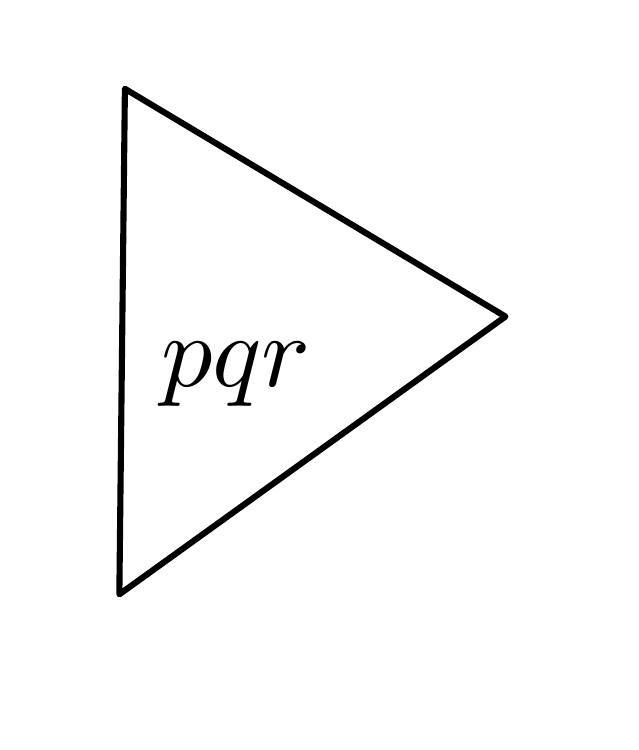
\begin{tikzpicture}[x=1bp,y=-1bp,line cap=round,line join=round]
\path[use as bounding box] (0,0) rectangle (210,250);
\begin{pgfinterruptboundingbox}
\draw[line width=2.2bp] (35,22) -- (172,104) -- (33,204) -- cycle;
\node[inner sep=0pt,outer sep=0pt,anchor=center] at (75,125) {\scalebox{3.7}{\ensuremath{pqr}}};
\end{pgfinterruptboundingbox}
\end{tikzpicture}
}\qquad Gleichung: $px+qy+rz=1$
\end{center}

% A544-P0320-D02
\begin{center}\emph{Coordinaten.}\end{center}
\begin{center}
\begin{minipage}{.28\textwidth}\centering
\resizebox{\linewidth}{!}{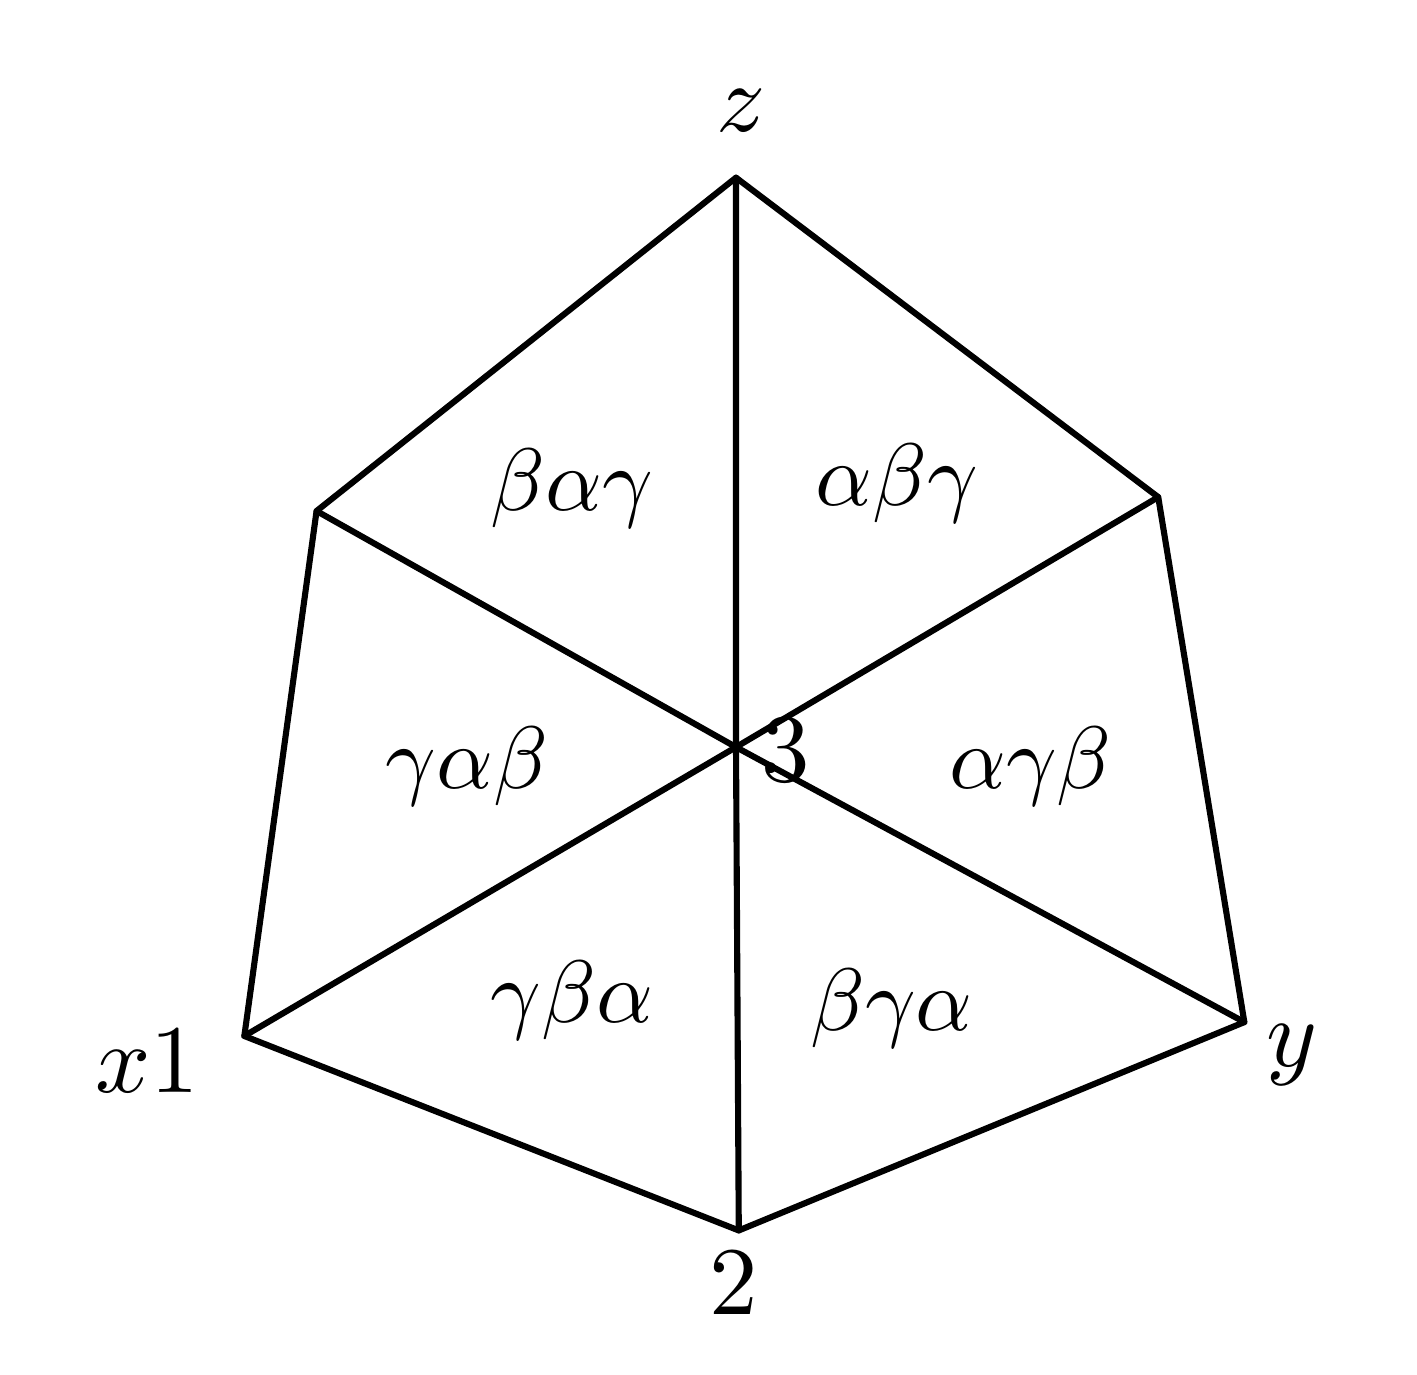
\begin{tikzpicture}[x=1bp,y=-1bp,line cap=round,line join=round]
\path[use as bounding box] (0,0) rectangle (490,475);
\begin{pgfinterruptboundingbox}
\draw[line width=2.2bp] (255,54) -- (407,169) -- (438,358) -- (256,433) -- (78,363) -- (104,174) -- cycle;
\draw[line width=2.2bp] (255,54) -- (255,259) -- (256,433);
\draw[line width=2.2bp] (104,174) -- (255,259) -- (438,358);
\draw[line width=2.2bp] (78,363) -- (255,259) -- (407,169);
\node[inner sep=0pt,outer sep=0pt,anchor=center] at (196,166) {\scalebox{3.2}{\ensuremath{\beta\alpha\gamma}}};
\node[inner sep=0pt,outer sep=0pt,anchor=center] at (313,164) {\scalebox{3.2}{\ensuremath{\alpha\beta\gamma}}};
\node[inner sep=0pt,outer sep=0pt,anchor=center] at (158,266) {\scalebox{3.2}{\ensuremath{\gamma\alpha\beta}}};
\node[inner sep=0pt,outer sep=0pt,anchor=center] at (361,266) {\scalebox{3.2}{\ensuremath{\alpha\gamma\beta}}};
\node[inner sep=0pt,outer sep=0pt,anchor=center] at (196,350) {\scalebox{3.2}{\ensuremath{\gamma\beta\alpha}}};
\node[inner sep=0pt,outer sep=0pt,anchor=center] at (311,353) {\scalebox{3.2}{\ensuremath{\beta\gamma\alpha}}};
\node[inner sep=0pt,outer sep=0pt,anchor=center] at (257,30) {\scalebox{3.5}{\ensuremath{z}}};
\node[inner sep=0pt,outer sep=0pt,anchor=center] at (43,372) {\scalebox{3.5}{\ensuremath{x1}}};
\node[inner sep=0pt,outer sep=0pt,anchor=center] at (455,370) {\scalebox{3.5}{\ensuremath{y}}};
\node[inner sep=0pt,outer sep=0pt,anchor=center] at (254,452) {\scalebox{3.5}{\ensuremath{2}}};
\node[inner sep=0pt,outer sep=0pt,anchor=center] at (273,260) {\scalebox{3.5}{\ensuremath{3}}};
\end{pgfinterruptboundingbox}
\end{tikzpicture}
}
\[\alpha<\beta<\gamma\]
\end{minipage}\hfill
\begin{minipage}{.68\textwidth}
\[
\begin{array}{rccc}
1.&\dfrac1\gamma&0&0\\[1ex]
2.&\dfrac1{\beta+\gamma}&\dfrac1{\beta+\gamma}&0\\[1ex]
3.&\dfrac1{\alpha+\beta+\gamma}&\dfrac1{\alpha+\beta+\gamma}&\dfrac1{\alpha+\beta+\gamma}
\end{array}
\]
\end{minipage}
\end{center}

% A544-P0320-D03
Sechsfacher Inhalt einer Elementarpyramide
\[
=\frac1{\gamma\pdot(\beta+\gamma)(\alpha+\beta+\gamma)}
\]
Alle [Flächen] sind um eine Kugel beschrieben, deren Halbmesser
\[
=\frac1{\surd(\alpha\alpha+\beta\beta+\gamma\gamma)}
\]
Doppelte Fläche eines Dreiecks
\[
=\frac{\surd(\alpha\alpha+\beta\beta+\gamma\gamma)}{\gamma(\beta+\gamma)(\alpha+\beta+\gamma)}
\]
Kante
\[
\begin{aligned}
1\pdot2&=\frac{\surd(\beta\beta+\gamma\gamma)}{\gamma(\beta+\gamma)},\\
1\pdot3&=\frac{\surd((\alpha+\beta)^2+2\gamma\gamma)}{\gamma(\alpha+\beta+\gamma)},\\
2\pdot3&=\frac{\surd(2\alpha\alpha+(\beta+\gamma)^2)}{(\beta+\gamma)(\alpha+\beta+\gamma)}
\end{aligned}
\]
Cosinus Kanten Winkel $3\pdot1\pdot2$
\[
=\frac{\alpha\beta+\beta\beta+\gamma\gamma}{\surd(\beta\beta+\gamma\gamma)((\alpha+\beta)^3+2\gamma\gamma)}
\]
Sinus
\[
=\frac{\gamma\pdot\surd(\alpha\alpha+\beta\beta+\gamma\gamma)}{\surd(\beta\beta+\gamma\gamma)((\alpha+\beta)^2+2\gamma\gamma)}
\]

% A544-P0320-D04
\begin{center}\emph{Vorkommende Werthe.}\end{center}
\begin{center}
\begin{tabular}{rccc l}
&$\alpha$&$\beta$&$\gamma$&\\
7.&0.&0.&1&Hexaeder\\
3.&0.&1.&1&Rhombendodekaeder\\
6.&0.&1.&2&Tetrakishexaeder\\
&0.&1.&3&\\
&0.&2.&3&\\
1.&1.&1.&1&Octaeder\\
5.&1.&1.&2&Trapezicositetraeder\\
&1.&1.&3&\\[1.2ex]
&$\alpha$&$\beta$&$\gamma$&\\
2.&1.&2.&2.&Triakisoctaeder\\
4.&1.&2.&3.&Hexakisoctaeder\\
&1.&2.&4.&\\
2.&1.&3.&3.&Triakisoctaeder\\
4.&1.&3.&5.&Hexakisoctaeder\\
2.&2.&3.&3&Triakisoctaeder\\
&2.&3.&4?&\\
&3.&5.&11&
\end{tabular}
\end{center}
\BookRule{.36\textwidth}

